\section*{Introduction}
Après plusieurs décennies de lente évolution, les réseaux électriques connaissent un développement
de grande envergure avec la multiplication des acteurs issus de la libéralisation des marchés
de l’énergie. Les préoccupations croissantes de sécurité d’approvisionnement et d’environnement,
les défis posés par le développement des énergies renouvelables et l’apparition de nouveaux usages
rendent les systèmes électriques de plus en plus complexes et donc vulnérables et plus chers en
exploitation. Lintroduction de plus d’intelligence grâce aux smart-grids est aujourd’hui le moyen
le plus efficace pour faire face à cette complexité croissante et résoudre les problèmes posés dans
les meilleures conditions de coût et de sûreté.

\begin{figure}[h]
	\centering
    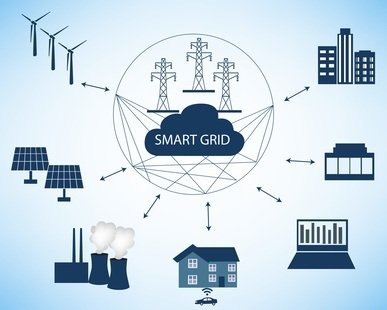
\includegraphics[scale=0.6]{img/part2/1.1}
    \caption{Le Smart Grid}
\end{figure}
